\PassOptionsToPackage{hidelinks}{hyperref}
\documentclass[doc,biblatex]{apa7}
\DeclareLanguageMapping{american}{american-apa}
\addbibresource{references.bib}
\captionsetup[figure]{textfont=rm,font=small,labelfont=bf}
\usepackage{amsmath}
\usepackage{mathspec}
\setallmainfonts{Times New Roman}
\setmainfont{Times New Roman}
% \setsansfont{Helvetica Neue}


\title{How does the writing system get informative? Differentiation or conservation?}

\shorttitle{Informativity in the writing system}

\authorsnames[1,1]{Jon W. Carr, Kathleen Rastle}

\authorsaffiliations{{Department of Psychology, Royal Holloway, University of London, England}}

% \authornote{\textbf{Cite as:} Carr, J.\@ W., \& Rastle, K.\@ (2023). Informativity in the writing system. \textit{OSF Preprints}. Version~0.}

\abstract{Abstract.}

\keywords{communication; cultural evolution; informativity; iterated learning; language evolution; orthography; spelling; sound change; writing}

\begin{document}

\maketitle

\noindent
Written languages represent spoken languages. However, there are many ways in which written languages diverge. E.g. spacing between words helps readers parse a sentence even if they are not technically required. Written languages can also have there own regularities such as spelling related words similarly (magician), past tense spellings directly conveying meaning, certain spellings conveying word class ous. These features abound in writing, especially in languages such as English that have not been subject to serious regulation.

One notable case of this is the heterographic homophones---words that sound alike but which are written with different spellings. For example, <meat> and <meet> are both pronounced /miːt/. Furthermore, these spellings can be cognitively useful . For example, faced with a sentence beginning /ðɛr/, a listener will have high uncertainty about what word---or even what sentence structure---is likely to come next: a noun, as in /ðɛr dɒg/, a form of the verb to be, as in /ðɛr ɪz/, or the progressive form of a verb, as in /ðɛr gəʊɪŋ/. In writing, by contrast, this uncertainty is greatly reduced; the spellings <their>, <there>, and <they're> differentiate between these cases, giving the reader a headstart on parsing the upcoming syntax. This idiosyncratic spelling of words that are homophonous in speech may confer certain benefits in reading, particularly in terms of comprehension. Heterography permits a writing system to be---at least in some areas---more informative than its spoken counterpart.

However, this additional informativeness comes at a cost. A system of words that conveys more information will---in general---be more complex than one that conveys less information. There exists a tradeoff between the simplicity of the spelling system and its ability to be expressive. A simple spelling system is one that is easy to learn, use, and process; for example, by being transparent with respect to phonology. The idea of a tradeoff between simplicity and informativeness in language structure has a longstanding history \parencite{Gabelentz:1891, Zipf:1949, Martinet:1952, Rosch:1978} and has recently been explored in a wide range of both typological \parencite{KempRegier:2012, Kemp:2018} and experimental \parencite{Carr:2020, Kirby:2015} studies. Of particular note here is the idea that the pressure for simplicity in language structure derives principally from learning, while the pressure for informativeness derives from the need for precise communication.

Any explanation for heterographic homophones must, therefore, demonstrate that heterographic spellings convey a benefit in terms of informativeness that is outweighed by the cost of learning the (often arbitrary) spelling distinction. What are the benefits? There seem to be broadly two kinds of benefit. (1) disambiguation in the writing of words that would otherwise be ambiguous if spelled transparently. (2) permitting the cognitive system to rapidly and accurately attain the meaning of a word. In this paper we limit ourselves to informativeness of the first kind, which is more amenable to experimental testing.

Is it possible, then, that heterography may be selected for in the cultural evolution of orthography? And if so, what might be the mechanism through which such selection could operate? \textcite[pp.~325--326]{Berg:2021} sketch two models of how a word might enter a state of heterography, as depicted in Fig.~\ref{models_of_heterography}. The first model, \textit{the differentiation model}, explains heterography through the creation of a new orthographic forms. For example, the word \textit{lite} is a respelling of \textit{light} frequently used in food products to distinguish light-in-calorific-weight from other meanings of \textit{light}; in British English, the word \textit{cheque} (perhaps influenced by \textit{exchequer}) differentiates the bank draft from other meanings of the word \textit{check}; and the word \textit{byte} was a deliberate respelling of \textit{bite} to avoid accidental mutation into the closely related term \textit{bit} \parencite{Buchholz:1977}. Etymological (and folk-etymological) spellings introduced during the Renaissance also occasionally resulted in heterographic homophones, perhaps contributing to their success: \textit{scene}--\textit{seen}, \textit{scent}--\textit{sent}, \textit{whole}--\textit{hole} \parencite[pp.~58--59]{Scragg:1974}, and many monosyllabic words that are homophonous with common function words have tended to adopt alternate spellings: \textit{be}--\textit{bee}, \textit{but}--\textit{butt}, \textit{by}--\textit{bye}--\textit{buy}, \textit{for}--\textit{fore}--\textit{four}, \textit{in}--\textit{inn}, \textit{or}--\textit{oar}--\textit{ore}, \textit{so}--\textit{sew}, \textit{to}--\textit{too}--\textit{two}, etc. Heterography is also very common in proper nouns: Surnames that are homophonous with common nouns often add <e> (\textit{Clarke}, \textit{Greene}, \textit{Wilde}) or double the final consonant (\textit{Carr}, \textit{Hogg}, \textit{Mann}), and it is common for brand names to adopt creative spellings, such as \textit{flickr}, \textit{Froot Loops}, or \textit{MVMT}.

	\begin{figure}
	\makebox[\textwidth][c]{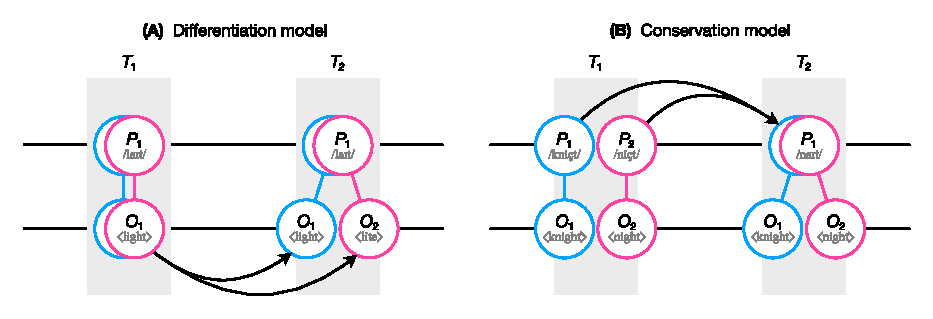
\includegraphics[]{figs/models_of_heterography.eps}}
	\vspace*{2pt}
	\caption{Two models of heterography. In the differentiation model, two meanings (represented by pink and blue) are, at time $T_1$, expressed by a single phonetic form $P_1$ and a single orthographic form $O_1$, but by time $T_2$, two orthographic forms have emerged to differentiate the meanings in writing. In the conservation model, the two distinct phonetic forms that existed at time $T_1$ have become homophonous by time $T_2$, but the two corresponding orthographic forms have been conserved, resulting in the same state of heterography as in the differentiation model. Adapted from \textcite[pp.~325--326]{Berg:2021} with permission.}
	\label{models_of_heterography}
	\end{figure}

The second model, \textit{the conservation model}, explains heterography as the historical residue of sound change: Two (or more) spoken forms merge and become homophonous, but the original heterographic spellings are conserved in the orthography. In English, for example, the meat--meet merger ultimately resulted in Middle English /ɛ:/ (spelled <ea>) and /e:/ (spelled <ee>) merging into /i:/ in Early Modern English, although the spellings were never updated accordingly, thus giving rise to a set heterographic homophones that persist in present-day English: \textit{heal}--\textit{heel}, \textit{leak}--\textit{leek}, \textit{meat}--\textit{meet}, \textit{read}--\textit{reed}, \textit{sea}--\textit{see}, \textit{team}--\textit{teem}, \textit{weak}--\textit{week}, etc. Similarly, other historic sound changes have likely resulted in (or contributed to) pairs of words entering a state of heterography, such as the reduction of /kn/ into /n/ (\textit{knight}--\textit{night}, \textit{know}--\textit{no}, \textit{knot}--\textit{not}, etc.), the loss of /ç/ (\textit{eight}--\textit{ate}, \textit{right}--\textit{rite}, \textit{sight}--\textit{site}, etc.), and the merger of /ʍ/ into /w/ (\textit{whale}--\textit{wail}, \textit{which}--\textit{witch}, \textit{whine}--\textit{wine}, etc.).

Processes

Sound change
dialect merger (bury is the spelling from one dialect with the pronunciation from another dialect)
Borrowing (English tends to retain spelling from the source language)
Printers innovations
- Etymological spellings (doubt)
- Deliberate design of heterographs
- Morphological spellings

\subsection{Research questions}

Q1) Does a learning pressure (induced through cultural transmission) result in the emergence of a simple, systematic, transparent orthography that is easier to learn? Hypotheses: In the high-variation conditions, where the orthography starts out chaotic (resulting in holistic systems), we expect simpler systems to emerge. Simplicity may be realized in a number of ways. Transparent systems use a one-to-one mapping to directly represent the spoken forms in writing. Redundant systems retain some spelling variation (with idiosyncratic spellings of the suffix for each shape) but become simpler by collapsing across colour. Expressive systems continue to express colour, but do so with a non-transparent but easy to learn compositional suffix system. The prevalence of these three types of system will be influenced by the presence of the communicative pressure. When communication is not present, transparent systems will tend to dominate, alongside some redundant systems and possibly some expressive systems. When communication is present, expressive systems will tend to dominate, perhaps with some redundant and holistic forms. The gradual emergence of simplicity, whatever form it takes, should be accompanied by increased learnability.

Q2) Can a writing system evolve to become more informative than its uninformative spoken counterpart? Hypotheses: Yes, but preferentially when two vital ingredients are present: a communicative pressure for informativeness (which makes an expressive system desirable) and high variation (which provides the building blocks to make that happen). When both ingredients are present, expressive systems will tend to dominate. If only one of the ingredients is available (either communication or high variation), informative systems may emerge but are less likely. In the case of learning-only and high-variation, expressive systems may emerge if the learners – yearning for an explanation for the variation – assume that colour must somehow be involved and therefore impose (perhaps unconsciously) colour-expressive structure on the language (i.e. learners may, to a certain extent, have a preconceived notion that languages ought to be informative). In the case of communication and no variation (where, again, only one of the ingredients is met), expressive systems may emerge but this is highly dependent on participants being 'innovators' who are willing to develop novel spelling systems that diverge from the spoken system in order to express colour. If neither ingredient is present, expressive systems will not emerge.



%~%~%~%~%~%~%~%~%~%~%~%~%~%~%~%~%~%~%~%~%~%~%~%~%~%~%~%~%~%~%~%~%~%~%~%~%~%~%~%~%~%~%~%~%~%~%~%~%~%~%~%

\section{Experiment 1}

Our first experiment tests the ability of the differentiation model to explain the emergence of informativeness in orthography. In particular we had two main hypotheses:

variation

communication

Preregistered \url{https://aspredicted.org/YLG_CKD}

\subsection{Methods}

To simulate the cultural evolution of orthography, we adopt the experimental iterated learning paradigm \parencite{Kirby:2008, Kirby:2015}. In this paradigm, some linguistic system is passed along a \textit{transmission chain} of human participants through repeated learning and production. Participant $i$ in the transmission chain learns the system based on the linguistic output of participant $i-i$ and then produces new linguistic output for participant $i+1$ to learn from. Through several \textit{generations} of this process, the linguistic system can gradually adapt to the learning biases of the human learners, yielding interesting emergent phenomena, such as compositionality \parencite{Kirby:2008, Kirby:2015}, combinatoriality \parencite{Verhoef:2015}, category structure \parencite{Carr:2017, Carr:2020}, and regularization \parencite{Smith:2010, Ferdinand:2019}.

To explore the hypotheses outlines above, we conducted the experiment under our different conditions: high variation vs.\@ no variation and communication vs.\@ no communication.

\subsubsection{Participants}

We recruited 538 participants via the Prolific platform. Participants were paid £3.00 for participation plus additional bonuses of up to £1.36 as detailed below (median bonus: £0.64). The median completion time was 19:36, resulting in an hourly rate of £9.18 (£11.03 including bonus). We limited recruitment to participants who had English as a first or second language to ensure they could understand the consent form and instructions; no other restrictions were applied. The most common first languages were: English (59\%), Polish (9.7\%), Portuguese (6.1\%), Italian (5.4\%), Spanish (5\%), and Greek (3.7\%). Five participants were rejected because they did not pass the random audio checks, and a further three participants were removed because they had been partnered with one of the five rejected participants. In addition, 35 participants were lost to communication-game pairing failures, resulting in a final dataset of 495 participants.

\subsubsection{Stimuli}

Participants were taught words for 16 ``alien'' objects---four shapes that could appear in four colors (see Fig.~\ref{}). The alien words had a spoken and written form composed of a stem and suffix. The stems, which express the shape dimension, were /buv/ <buv>, /zɛt/ <zet>, /gaf/ <gaf>, and /wɒp/ <wop>. Since we are not interested in participants' learning of the stems, they were designed to be quick and easy to learn by being graphically and phonetically iconic of the shapes they represent, and they were fixed and unchanging throughout the experiment. The suffix was always pronounced /ikəʊ/ in speech, but its spelling was free to change over time. Thus, the spoken form of the language consists of just four unique words---/buvikəʊ/, /zɛtikəʊ/, /gafikəʊ/, and /wɒpikəʊ/---that mark a shape distinction; however, the \textit{spelling} of the suffix could potentially take on different forms to mark color. The spoken forms were synthesized using the Apple text-to-speech synthesizer (the Tessa voice).

The transmission chains were seeded with an orthographic system that may exhibit high variation or no variation according to condition. In the no-variation conditions, the suffix had only one spelling, although each chain was initialized with a different randomly generated spelling. To generate a spelling we randomly choose a grapheme from each of the sets \{<ee>, <i>, <y>\}, \{<c>, <ck>, <k>\}, and \{<oe>, <oh>, <ow>\} and concatenate them. For example, in one chain the suffix might initially be spelled <icoe>, while in another chain it might initially be spelled <yckow>. In the high-variation conditions, the spellings were randomly generated not just for each chain but also for each of the 16 objects. Thus, although the star shaped objects are all called /zɛtikəʊ/ in speech, the different colors have different random spellings (e.g., <zetikow> for pink, <zeticoe> for gray, <zeteeckoe> for blue, and <zetyckoh> for yellow). These spellings were not systematic, however; for example, the <yckoh> spelling was not systematically used to represent yellow across different shapes. Essentially, then, in the no-variation conditions there is initially only one possible way to spell /ikəʊ/, while in the high-variation conditions there are many possible ways to spell it without any systematic pattern.

\subsubsection{Transmission procedure}

As outlined above, the participants were arranged into transmission chains such that the spellings produced by one participant would subsequently be taught to the next participant in the chain. The first participant in a chain was taught the initial, randomly generated orthographic system, and this system was then free to evolve as it was culturally transmitted. This was subject to a bottleneck on transmission: Not all 16 spellings were transmitted from one generation to the next; rather, the participant at generation $i$ would observe only 12 of the 16 spellings generated at generation $i-1$ (at least one of each shape and at least one of each color). Transmission continued until the chain converged on a particular orthographic system. A chain is said to converge when two consecutive generations produce identical spellings for all 16 items (including the four unseen items), suggesting that the chain is unlikely to experience significant further change. We adopted this convergence-based approach because we were primarily interested in revealing what kinds of orthographic system are stable under the four conditions, but it was unclear a~priori how many generations would be required to reveal this information.

\subsubsection{Training procedure}

Participants were trained on the spoken and written forms through a combination of passive exposure trials and ``mini-test'' trials. In the passive exposure trials, the alien object was presented alongside the written and spoken forms for 2000~ms. The written form appeared after a 500~ms delay so that participants would first attend to the object before looking at the word. In mini-test trials, which were interleaved among the passive exposure trials, the participant had to type in the appropriate written form for one of the objects. The mini-tests were included to help participants actively engage in the learning process. After submitting a spelling, the participant was given feedback on any errors (additions shown in bold green text and deletions shown in red strikethrough text). The input box only accepted lowercase alphabetical strings of between four and nine characters, and spellings containing certain letter combinations (e.g., <bk>, <bl>, <pin>, <ye>) were not accepted to prevent participants from entering English color words or abbreviations thereof. Participants received a 1p bonus for spelling the stem correctly or a 2p bonus for spelling the entire word correctly. However, to receive the bonus, their response had to be submitted within 20~seconds. Each of the 12 object--word pairs in the training set (i.e., those that passed through the bottleneck on transmission) was passively exposed 12 times and mini-tested 3 times, resulting in a total of 144 passive exposure trials and 36 mini-test trials (the maximum possible bonus in training was therefore 72p). To ensure that participants were indeed listening to the spoken forms, a voice asked participants to click on the object at three random points during training; participants who did not follow this instruction were excluded.

\subsubsection{Non-communicative test procedure}

After training, participants assigned to the non-communicative conditions completed a test phase, alternating between two types of test trial, production trials and comprehension trials. In production trials, the participant was shown an object and heard its associated word pronounced aloud. The task was to type~in the appropriate spelling under the same input restrictions as in mini-test trials and an additional restriction that the stem (i.e., the first three letters of the word) had to be spelled correctly to ensure that stems could not diverge from the spoken forms over time. Since participants heard the word pronounced aloud, typing the stem correctly should be trivial, but in cases where the stem was initially spelled incorrectly, a popup message explicitly told the participant the correct spelling of the stem. In comprehension trials, the participant was shown a word and had to click on the matching object from all 16 objects arranged in random order (in cases where multiple objects were described by the same wordform, any of the objects was a valid choice). In both types of test trial, the participant was awarded a bonus of 2p for every correct answer (unlike mini-tests, there was no 1p bonus for partially correct spellings). Each of the 16 object--word pairs (i.e., including the four unseen items) was tested once in production and once in comprehension, resulting in 32 trials and a maximum bonus of 64p. Binary feedback was provided on each trial in the form of a sound effect.

\subsubsection{Communicative test procedure}

After training, participants assigned to the communicative conditions completed a live, over-the-internet communication game with another participant. The two participants both received training on the same orthographic system inherited from a previous generation, albeit subject to independent bottlenecks on transmission. The communication game mirrors the overall structure of the non-communicative test with the production and comprehension trials becoming the two sides of a communicative interaction. On a given trial, one participant---the sender---would complete a production trial (produce a word for a given meaning) and this word was transmitted to the other participant. The second participant---the receiver---would then complete a comprehension trial (select an object for the received word). The participants then switched roles, resulting in the same overall trial structure as the non-communicative condition (i.e., alternation between production and comprehension trials with the same bonusing scheme). However, the communication game differed from the non-communicative test in three ways. First, the transmitted and received words were displayed in text message speech bubbles to emphasize the communicative nature of the test. Second, in cases where a single wordform maps to multiple objects, the receiver performing the comprehension trial could not click any of the objects---their goal was to click the target object being communicated by the sender. Third, both participants received rich feedback: The sender saw which object the receiver clicked on, and the receiver saw which object was the correct target. Overall, then, the communicative test is identical to the non-communicative test in terms of the task to be performed, but the goal is quite different: In the non-communicative test, the goal and reward structure is based on accurately reproducing the orthography learned during training, whereas in the communicative test, the goal and reward structure is based on successfully communicating a target item.

\subsection{Results}

Learnability, measured as transmission error (lower error = higher learnability). Mean Levenshtein edit distance between the words produced at generation i and the corresponding words produced at generation i-1.

Simplicity, measured as complexity (lower complexity = higher simplicity). The length (in bits) of the shortest grammar that losslessly compresses the lexicon, as computed by the Grammarette package: https://github.com/jwcarr/grammarette. Finding the shortest grammar for some lexicon is a non-trivial problem, and it is likely that we will need to adapt the method in response to the collected data.

Communicative cost is given by
\begin{equation}
\mathrm{cost}(L) := \frac{1}{|U|} \sum_{m \in U} -\log \mathrm{Pr}(m|s_m),
\end{equation}
where $\mathrm{Pr}(m|s_m)$ is the probability that a listener would infer meaning $m$ given that a speaker produced signal $s$ for meaning $m$. Here we assume this probability to be $1/|M_s|$, where $M_s$ is the set of meanings labeled $s$.


For the purpose of the results, we are primarily interested in the spelling of the suffixes, so we first needed to isolate the suffixes from the stems. Although the first three letters (<buv>, <zet>, <gaf>, <wop>) were fixed and unchanging throughout the experiment, it was possible for the stems to grow longer if additional material was inserted before the suffix (e.g., <gaff>, <wopb>, <zetch>). We consider the stem to be all material up to but not including the first vowel letter after the original three-letter stems, such that, for example, <zethyckoh> will be parsed into the stem <zeth> and suffix <yckoh>. Of course, it is not possible to know how participants themselves divided the strings (if at all), but since all words were phonetically identical from the /i/ vowel onward, it is reasonable to parse the strings this way on the basis that this yields the shortest grammar.

To analyze the variation in the suffix spellings and how it correlates with meaning, each participant's system was transformed into a 4×4 matrix, with rows representing the shape dimension, columns representing the color dimension, and the matrix values representing the unique spellings. For example, a ``degenerate'' system of suffix spellings---one that uses a single spelling for all meanings---would have the following matrix representation:
\begin{equation}
	S_\mathrm{degenerate} = \begin{bmatrix}
	1 & 1 & 1 & 1 \\
	1 & 1 & 1 & 1 \\
	1 & 1 & 1 & 1 \\
	1 & 1 & 1 & 1
	\end{bmatrix}
\end{equation}
Here the number 1 represents the one and only suffix spelling. We define an ``expressive'' system as one that marks the color dimension using four distinct spellings, resulting in the following matrix:
\begin{equation}
	S_\mathrm{expressive} = \begin{bmatrix}
	1 & 2 & 3 & 4 \\
	1 & 2 & 3 & 4 \\
	1 & 2 & 3 & 4 \\
	1 & 2 & 3 & 4
	\end{bmatrix}
\end{equation}
In such a system, although the suffix only expresses color, the words as a whole are fully informative, since shape is expressed by the stem. A third system of interest is the ``redundant'' system:
\begin{equation}
	S_\mathrm{redundant} = \begin{bmatrix}
	1 & 1 & 1 & 1 \\
	2 & 2 & 2 & 2 \\
	3 & 3 & 3 & 3 \\
	4 & 4 & 4 & 4
	\end{bmatrix}
\end{equation}
Although $S_\mathrm{redundant}$ carries the same amount of information as $S_\mathrm{expressive}$, it marks a dimension (shape) that is already expressed by the stem, making the information carried by the suffix redundant. Such a system contains unnecessary complexity---different ways of writing /ikəʊ/ that carry no additional information.

Of course, the suffix spelling systems produced by participants may not match these three reference systems exactly. To determine which reference system a participant's output system is most similar to, we adopt variation of information \parencite[VoI;][]{Meila:2007} as a distance metric. VoI is a proper metric on set partitions, measuring the amount of information (in bits) that is lost and gained in the transformation of one set partition into another set partition. So, for example, the distance between $S_\mathrm{degenerate}$ and $S_\mathrm{expressive}$ is 2~bits because $S_\mathrm{expressive}$ conveys 2~bits of information\footnote{In $S_\mathrm{expressive}$, knowing the suffix reduces uncertainty from 16 equally probable meanings to 4 equally probable meanings; $-\log\frac{4}{16} = 2$~bits.}, 2~bits more than $S_\mathrm{degenerate}$, which conveys 0~bits of information. The distance between $S_\mathrm{expressive}$ and $S_\mathrm{redundant}$ is 4~bits; this is because, although both systems convey 2~bits of information, the information they convey is entirely orthogonal; in switching from $S_\mathrm{expressive}$ to $S_\mathrm{redundant}$, one loses 2~bits of information (information about color), but one gains 2~bits of information (information about shape), making the total distance 4~bits.

We computed the VoI between the emergent suffix systems and the three reference systems and plotted them on a ternary diagram, the three vertices of which represent the three reference systems (see Fig.~\ref{exp1_ternary_plot}). The diagram is divided into three sectors (shades of gray), which reveal which reference system the final converged-on suffix systems are most similar to. Most of the emergent system are either redundant or degenerate, with some straddling the border between the two. No system is classified as expressive, although two of the converged-on systems (highlighted in Fig.~\ref{exp1_ternary_plot}) showed some signs of color-marking. In one system, <icoe> is used for gray objects and <ikoe> for all other colors. In the other system, <ikcow> is used for gray objects and <ikoe> is used for all other colors, except the star shape uses <y> instead of <i> (i.e., <ykcow> and <ykoe>), resulting in some spelling redundancy\footnote{However, rather than parsing the stems as <buv>, <zett>, <gaf>, <wop>, they could instead be parsed as <buvi>, <zetty>, <gafi>, <wopi>. Under this interpretation, there would be no redundancy and the system would be equivalent to the other 1-color emergent system.} In general, there is no discernible difference between the two conditions; regardless of whether the communicative pressure was present, the emergent suffix spelling systems tended to fall along the degenerate--redundant axis, and the only two cases of color-marking were in~fact from the learning-only condition.

\subsection{Summary}

Our first experiment tested the ability of the differentiation model to explain the emergence of an informative, heterographic orthography, but we found little evidence of systematic orthographic differentiation. Exposed to an orthography with high variation, learners could have gradually conditioned that variation on the dimension where it would have been useful from the point of view of disambiguation, color, yielding differentiated forms in the orthography. But this did not happen, even under the communicative pressure. Instead, when spelling variation was conditioned on anything, it was conditioned on shape, resulting in redundant suffix spellings. This result is in stark contrast to most prior experimental iterated learning studies, in which informative, compositional systems do typically emerge, especially under communicative pressure. So, what was different about the present experiment? The primary difference was the presence of a spoken language that is decidedly \textit{not} informative, which acts as a cue to participants that the language does not mark color and that, therefore, the orthography should not mark color. Faced with variation that could be conditioned on shape or color, learners rule out the possibility that it might be conditioned on color, since such a hypothesis would be in conflict with the spoken language. As a result, variation in spelling comes to be associated with particular stems, resulting in the emergence of idiosyncratic suffix spellings that serve no real purpose. A rough analog of this redundancy can be found in English in the spelling of the /ʃən/ suffix (<cian>, <sion>, <ssion>, or <tion>), which is largely conditioned on the stem (e.g., \textit{magician}, \textit{expansion} \textit{transmission}, and \textit{invention}).

Another pathway through which differentiation could have occurred is through conscious innovation, especially in the communicative conditions, where participants could have increased their bonuses substantially by innovating a system of color markers. However, there was no evidence of such innovation, and only four participants mentioned that they even \textit{considered} this possibility in their post-test comments (e.g., ``I wondered if I should use the color suffix rule even where I did not think it was the right word to try and help my partner get the right color object''). Why do participants choose not to innovate or even regularize an imperfect system? Firstly, although innovation was not expressly forbidden, it was perhaps suggested by the overall structure of the experiment that we expected them to use the orthography learned during training. Participants who adopted this interpretation may have feared diverging from their training either because they themselves wanted to avoid breaking the rules or because they did not know whether their partner would feel comfortable breaking the rules. Secondly, even if participants are willing to diverge, they are presented with an alignment problem: How can they decide what system of color marking to use when there is no channel through which they can have a meta-discussion? They can only use trial-and-error, and even then, the process is complicated by participants simultaneously adapting to each other's systems. Interestingly, these are dynamics that also exist in the real world, where deviation from received, sacrosanct spellings is considered socially unacceptable or uneducated (e.g., the non-standard spelling <thru> has struggled for decades---or perhaps centuries---to make any headway against <through>), and even under more progressive attitudes to change and innovation, the problem of achieving community buy-in remains, especially when the change is not imposed by top-down authority: If I decided to start using the spelling <banque> to differentiate the financial institution from river banks, would anyone take my spelling seriously or even understand the distinction I was trying to make?

Overall, our first experiment suggests that differentiation---be it through a self-organizing process in learning or through a conscious process of innovation in use---is not a good model of heterography, unless enforced by top-down authority. We now turn to consider the conservation model.

%~%~%~%~%~%~%~%~%~%~%~%~%~%~%~%~%~%~%~%~%~%~%~%~%~%~%~%~%~%~%~%~%~%~%~%~%~%~%~%~%~%~%~%~%~%~%~%~%~%~%~%

\section{Experiment 2}

Our second experiment investigates the conservation model: Given than an informative system already exists (both in speech and in writing), will the informative system persist even after the degeneration of the spoken language towards homophony? And does this happen preferentially in the presence of a shared communicative task. How much homophony can an informative, heterographic system resist under an increasingly strong simplicity pressure.

\subsection{Methods}

The methods were identical to Experiment~1 with the following major exceptions. Firstly, and most notably, the artificial language used to seed each chain starts out fully compositional (in both its spoken and written forms), since we are now interested in whether the orthographies will maintain informativeness rather than gain it. Secondly, and consequently, the convergence-based approach used in Experiment~1 to determine the number of generations is no longer appropriate, so we now use a fixed number of generations. Thirdly, we simulate regular sound mergers which result in the spoken forms of the suffixes becoming increasingly less informative over generational time (this contrasts with Experiment~1, where the spoken form of the suffixes were always fully uninformative).

\subsubsection{Participants}

We recruited xxx participants via the Prolific platform. The payment and bonusing scheme was identical to Experiment~1 (median bonus: £0.xxx). The median completion time was xxx:xxx, resulting in an hourly rate of £xxx (£xxx including bonus). Unlike Experiment~1 we restricted recruitment to native speakers of English because it was particularly important that participants would be able to distinguish the voiceless fricatives /θ s ʃ h/ and we found in piloting that non-native speakers of English frequently struggled with these distinctions. xxx participants were rejected because they did not pass the random audio checks, and a further xxx participants were removed because they had been partnered with one of the rejected participants. In addition, xxx participants were lost to communication-game pairing failures, resulting in a final dataset of 360 participants (organized into ten chains of twelve generations in each condition, with two participants per generation in Learning \& Communication).

\subsubsection{Stimuli}

The alien objects and word stems were identical to Experiment~1. Unlike Experiment~1, however, the chains were initialized with a fully compositional language that uses four distinct suffixes to systematically express each of the four colors. The suffixes took the form /ɪ\textit{CV}/ where $C$ is a voiceless fricative consonant from the set \{/θ/, /s/, /ʃ/, /h/\} and $V$ is a vowel from the set \{/ə/, /ɛɪ/, /əʊ/, /u/\}. The consonant and vowel sets were randomly permuted for each iterated learning chain, such that the suffix forms were unique to each chain. For example, under the permutations given above, the resulting suffixes would be /ɪθə/, /ɪsɛɪ/, /ɪʃəʊ/, and /ɪhu/, but another iterated learning chain might use the suffixes /ɪsəʊ/, /ɪʃɛɪ/, /ɪθu/, and /ɪhə/. The initial orthographic system used to seed the chain was generated based on the following phoneme–grapheme mapping \{/θ/→<th>, /s/→<s>, /ʃ/→<sh>, /h/→<x>, /ə/→<a>, /ɛɪ/→<e>, /əʊ/→<o>, /u/→<u>\}. The suffixes were designed to be distinctive (and therefore easy to memorize and recall), but also similar enough to (mostly) allow for somewhat plausible sound mergers and result in somewhat plausible spellings following sound merger (e.g., it is plausible that /θ/ might be supplanted by /s/ in speech or that /θ/ might be spelled <x> in writing). We attempted to achieve this balance by combining consonants that are very similar (differing only in place of articulation) with vowels that are very dissimilar.

\subsubsection{Sound change}

Each iterated learning chain was run for 12 generations, divided into four epochs of three generations. In the first epoch, all spoken suffixes were distinct, allowing the spoken language to express all four colors, but by the fourth epoch all suffixes were reduced into a single phonetic form, making the spoken language entirely uninformative about color. This was achieved through three sound changes occurring between the four epochs. In the first sound change, two of the suffixes were chosen at random to be merged. To perform the merger, the consonant from one of the suffixes (chosen at random) was paired with the vowel from the other suffix, resulting in a new suffix form that would replace the original two. For example, assuming the language has the suffixes /ɪθə/ (pink), /ɪsɛɪ/ (gray), /ɪʃəʊ/ (blue), and /ɪhu/ (yellow), we might merge /ɪsɛɪ/ and /ɪhu/ into /ɪhɛɪ/, such that the spoken language is no longer able to mark a distinction between gray and yellow. In the second sound change, the same procedure is applied to the two suffixes that were not selected previously (e.g., /ɪθə/ and /ɪʃəʊ/ become /ɪθəʊ/). And in the third and final sound change, the two suffix forms created through the first and second sounds changes---/ɪhɛɪ/ (grey/yellow) and /ɪθəʊ/ (pink/blue)---merge into a single form (e.g., /ɪθɛɪ/). Importantly, the spellings do not change automatically following a sound change event; instead, the orthographic system is free to adapt (or not) in response to sound changes.

\subsection{Results}



\subsection{Summary}

%~%~%~%~%~%~%~%~%~%~%~%~%~%~%~%~%~%~%~%~%~%~%~%~%~%~%~%~%~%~%~%~%~%~%~%~%~%~%~%~%~%~%~%~%~%~%~%~%~%~%~%

\section{Discussion}

%~%~%~%~%~%~%~%~%~%~%~%~%~%~%~%~%~%~%~%~%~%~%~%~%~%~%~%~%~%~%~%~%~%~%~%~%~%~%~%~%~%~%~%~%~%~%~%~%~%~%~%

\section{Acknowledgments}

\noindent This work was funded by a grant from the Leverhulme Trust.

\printbibliography

\end{document}